\documentclass{beamer}

\usepackage[all]{xy}
\usepackage{listings}
\usepackage{slashbox}
\usepackage{booktabs}
\usepackage{amsmath,amssymb}
\usepackage{hyperref}
\usepackage{graphicx}

\DeclareMathOperator*{\argmin}{arg\,min}
\DeclareMathOperator*{\argmax}{arg\,max}
\DeclareMathOperator*{\maximize}{maximize}
\DeclareMathOperator*{\minimize}{minimize}
\newcommand{\sign}{\operatorname{sign}}
\newcommand{\RR}{\mathbb R}
\newcommand{\NN}{\mathbb N}

\AtBeginSection[]
{
  \begin{frame}
    \tableofcontents
  \end{frame}
}

\begin{document}

\title{Organizing computational research projects}
\author{
Toby Dylan Hocking\\
tdhock5@gmail.com
}

\date{20 Feb 2014}

\maketitle

\begin{frame}
  \frametitle{Motivation: reproducible computations}
  \begin{displaymath}
\xymatrix{
  \text{Laboratory}
  \ar[r]^{\text{notebook}}_{\text{experiments}}
&
  \text{computer files}
  \ar[r]^{\fbox{\text{XXXXX}}}_{\text{computations}}
  &
  \text{research article}
}
  \end{displaymath}
  \begin{itemize}
  \item Lab notebooks essential for reproducible experiments.
  \item Lab notebooks skills are taught in school.
  \item \fbox{XXXXX} essential for reproducible computations.
  \item \fbox{XXXXX} skills are NOT taught.
  \end{itemize}
\end{frame}

\begin{frame}
  \frametitle{A quick guide to organizing computational biology
    projects}
  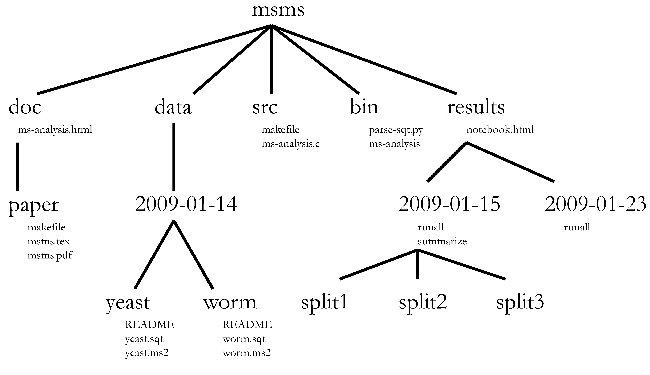
\includegraphics[width=\textwidth]{figure-noble-directories-nohilite}

  Source: William Stafford Noble, PLoS Comp Bio 2009.
\end{frame}

\begin{frame}
  \frametitle{Human-readable files (notes to future self)}
  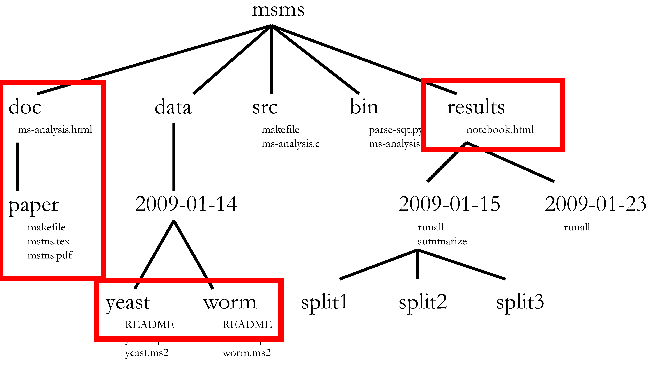
\includegraphics[width=\textwidth]{figure-noble-directories-docs}

  Source: William Stafford Noble, PLoS Comp Bio 2009.
\end{frame}

\begin{frame}
  \frametitle{Computer-readable files (reproducible computations)}
  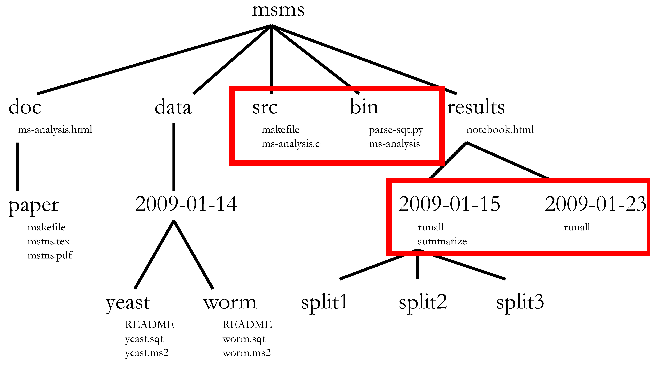
\includegraphics[width=\textwidth]{figure-noble-directories-scripts}

  Source: William Stafford Noble, PLoS Comp Bio 2009.
\end{frame}

\begin{frame}
  \frametitle{Without version control you can easily get}
  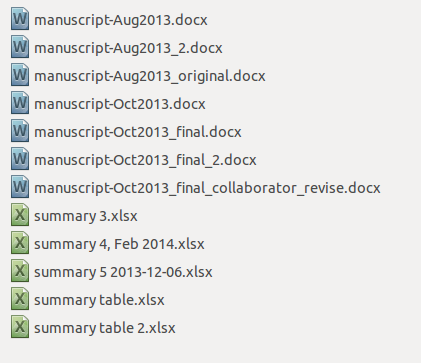
\includegraphics[width=\textwidth]{screenshot-avoid}
\end{frame}

% \begin{frame}
%   \frametitle{A Makefile facilitates reproducible computations}
%   Just type \texttt{make} ...

%   TODO: command line example change a figure source file.
% \end{frame}

\begin{frame}
  \frametitle{With version control you get}
  \begin{itemize}
  \item Backup.
  \item Go back in time.
  \item Collaboration.
  \end{itemize}
  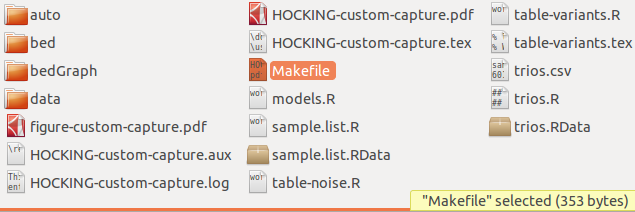
\includegraphics[width=4in]{screenshot-makefile}  
\end{frame}

\begin{frame}[fragile]
  \frametitle{I use a Makefile for each of my projects}
  % Write what to compute/plot/show in R/\LaTeX/etc.
  % \begin{itemize}
  % \item Record each computation in R code files.
  % \item R code exports result figures and tables.
  % \item Write the manuscript in a \LaTeX\ file.
  % \end{itemize}
  Write relations between files as rules in a Makefile:
  \begin{itemize}
  \item For each computation/figure/table, save 1 file (the target).
  \item Write what files are required (the prerequisites).
  \item Write a command line to do it (the recipe).
  \end{itemize}
\begin{verbatim}
thocking@silene$ make figure-3.png
thocking@silene$ make table-1.tex
thocking@silene$ make notebook.pdf
thokcing@silene$ make 
\end{verbatim}
Note: last line means make first target in the Makefile.
\end{frame}

% \begin{frame}
%   \frametitle{Scriptable, free/open-source programs}
%   \begin{tabular}{lll}
%     Program & since & like \\
%     \hline 
%     \LaTeX & 1978 & 
%   \end{tabular}
% \end{frame}

\begin{frame}
  \frametitle{A Makefile records how to compute each project file}
  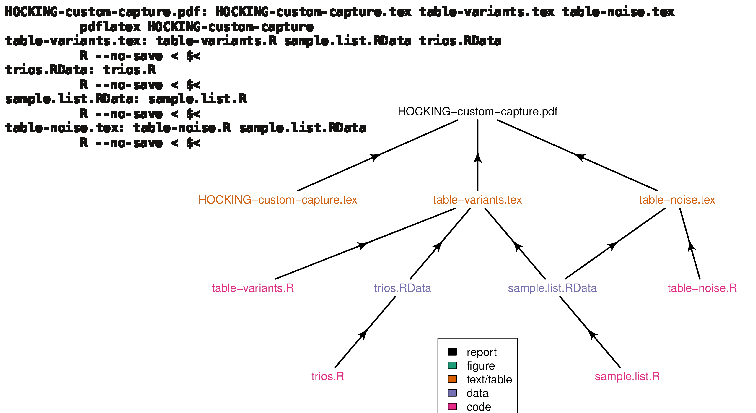
\includegraphics[width=\textwidth]{figure-code-dag}
\end{frame}

\begin{frame}
  \frametitle{A Makefile contains a rule for each computed file}
  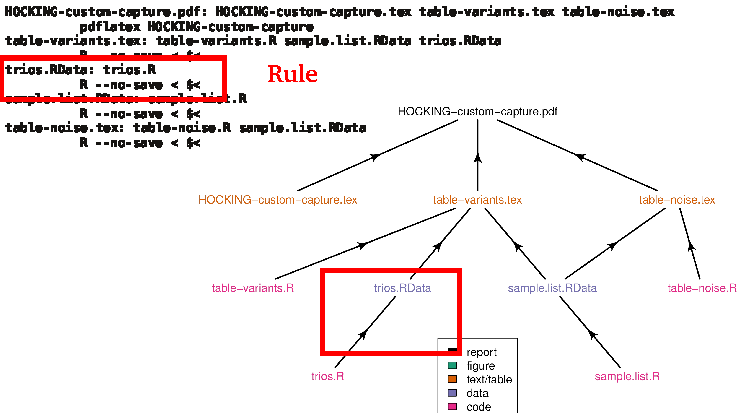
\includegraphics[width=\textwidth]{figure-code-dag-line3}
\end{frame}

\begin{frame}
  \frametitle{The computed file is called the target}
  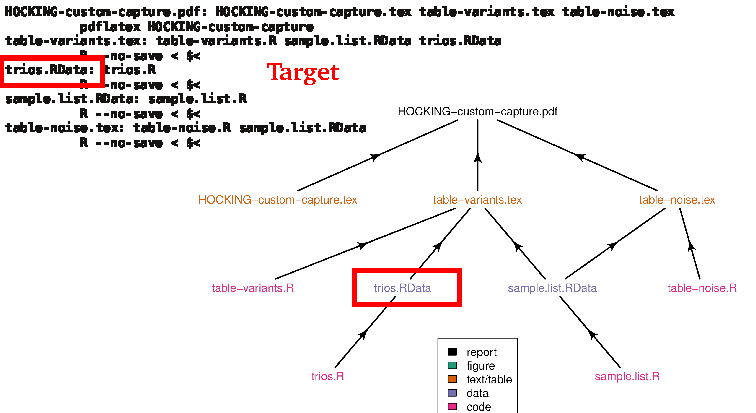
\includegraphics[width=\textwidth]{figure-code-dag-line3-target}
\end{frame}

\begin{frame}
  \frametitle{The input files are called prerequisities}
  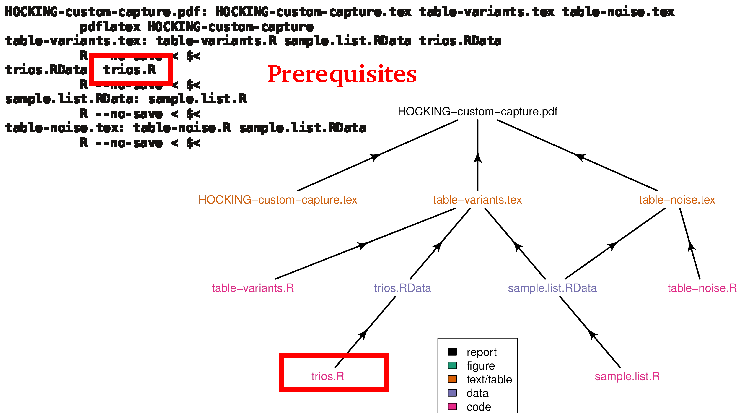
\includegraphics[width=\textwidth]{figure-code-dag-line3-prerequisites}
\end{frame}

\begin{frame}
  \frametitle{The recipe is the command line used to compute}
  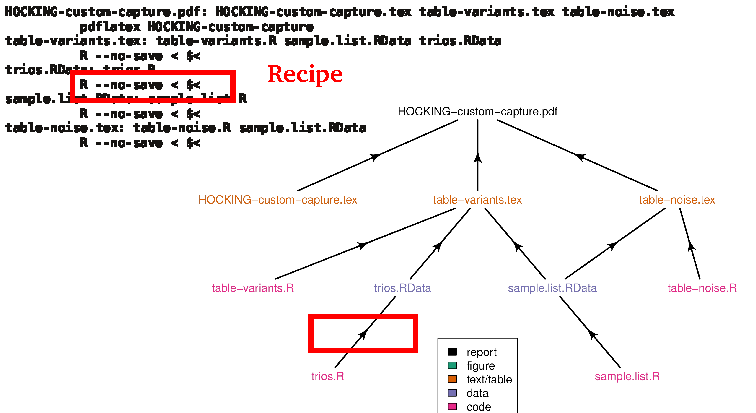
\includegraphics[width=\textwidth]{figure-code-dag-line3-recipe}
\end{frame}

\begin{frame}
  \frametitle{Make provides abbreviations to avoid repetition}
  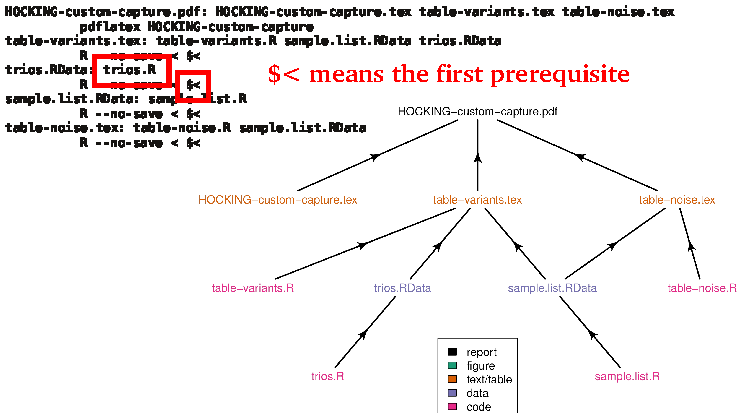
\includegraphics[width=\textwidth]{figure-code-dag-line3-abbrev}
\end{frame}

\begin{frame}
  \frametitle{Read slow CSV data and save in fast RData format}
  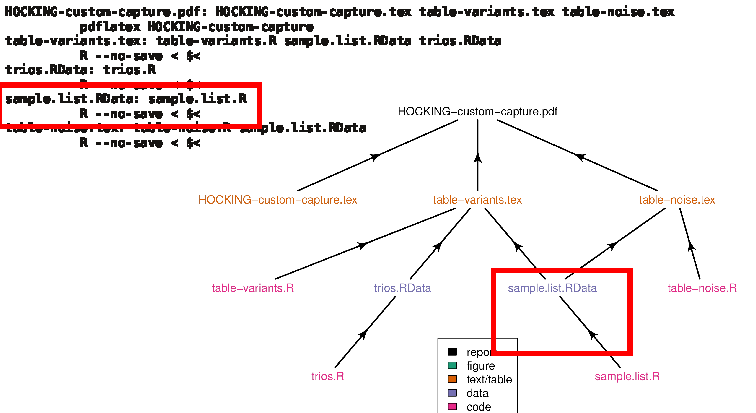
\includegraphics[width=\textwidth]{figure-code-dag-line4}
\end{frame}

\begin{frame}
  \frametitle{Table of genes that were excluded as noise}
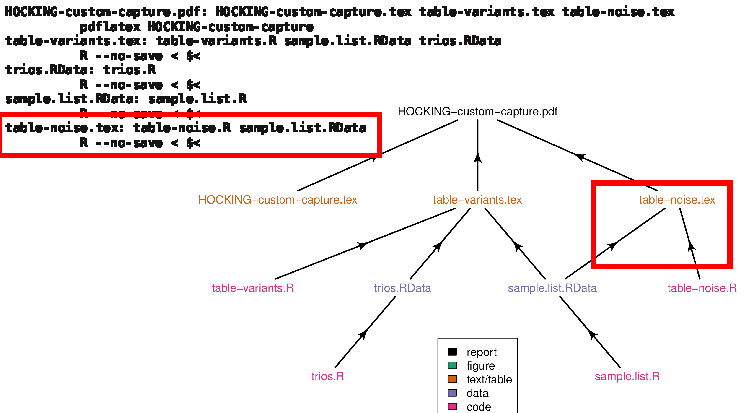
\includegraphics[width=\textwidth]{figure-code-dag-line5}
\end{frame}

\begin{frame}
  \frametitle{Table of detected variants for every sample}
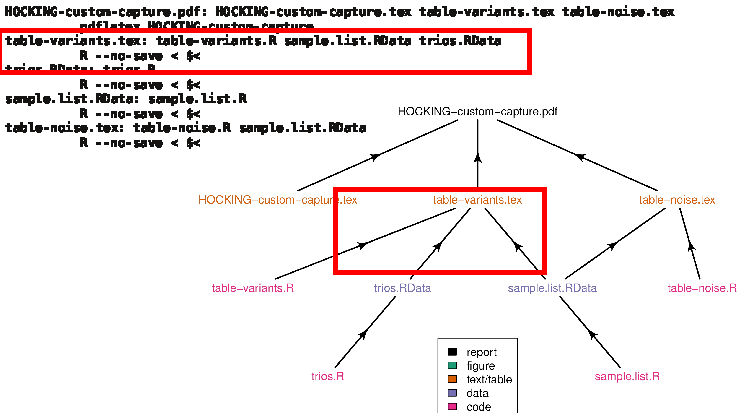
\includegraphics[width=\textwidth]{figure-code-dag-line2}
\end{frame}

\begin{frame}
  \frametitle{A recipe can produce more files if necessary}
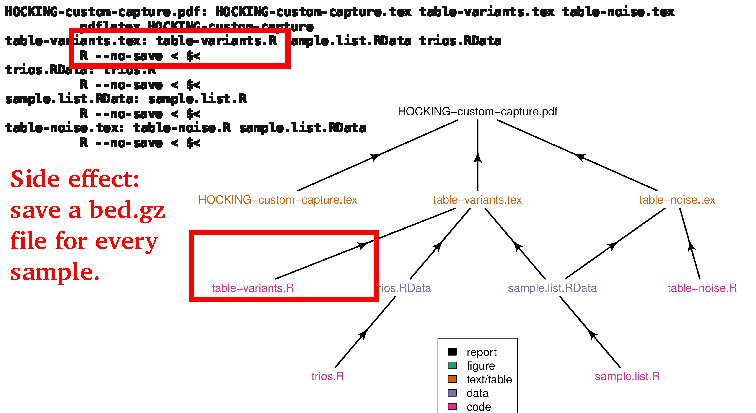
\includegraphics[width=\textwidth]{figure-code-dag-line2-bed}
\end{frame}

\begin{frame}
  \frametitle{The final report PDF with computed data tables}
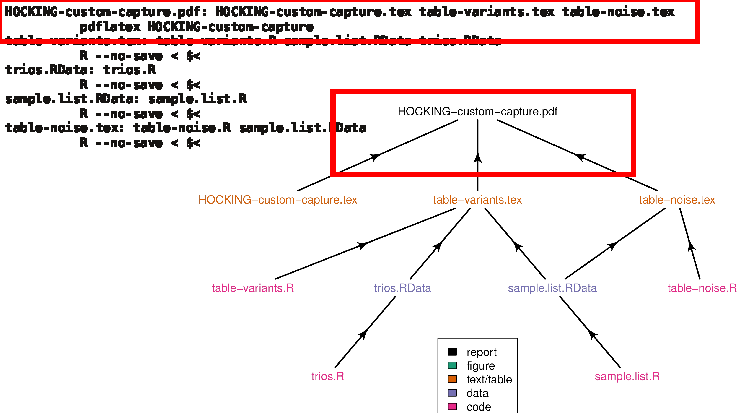
\includegraphics[width=\textwidth]{figure-code-dag-line1}
\end{frame}

\begin{frame}
  \frametitle{Limitations}
  \begin{itemize}
  \item You need to write R/\LaTeX\ code (complicated).
  \item Really big files/calculations?
  \item Where to record software versions?
    \texttt{install.packages("changepoint")} vs
    \texttt{works\_with\_R("3.0.2", changepoint="1.1.1")}
  \end{itemize}
\end{frame}

\end{document}
